\section{\label{sec:GWs}Gravitational Waves}

This section will reproduce the derivation of \gws, closely following the textbook `A General Relativity Workbook' by Thomas A. Moore \cite{moore_2013}.

General Relativity (GR) is our current theory of gravitation in the Universe. GR introduces the Einstein field equations (EFEs), described by equation \ref{eqn:EFE}, which relate the curvature of spacetime to the matter and energy
within it. Solving EFEs is extremely difficult to do analytically so we must resort to looking at heavily simplified problems or using numerical relativity and the power of supercomputers.

\begin{equation}
   G^{\mu \nu} = 8 \pi G T^{\mu \nu}
   \label{eqn:EFE}
\end{equation}

Where $G^{\mu \nu}$ is the Einstein tensor, $G$ is Newton's constant of gravitation and, $T^{\mu \nu}$ is the stress-energy tensor.

One of the predictions of GR is the existence of \gws. To derive \gws with the Einstein field equations, we must begin with some assumptions about our spacetime. Far from the source of \gws, where the stress-energy tensor
$T^{\mu \nu} = 0$, we can describe the spacetime as flat with a tiny perturbation caused by the presence of \gws. Our metric can be described as follows:

\begin{equation}
   g_{\mu \nu} = \eta_{\mu \nu} + h_{\mu \nu}
   \label{eqn:g_mu_nu}
\end{equation}

Where $\eta_{\mu \nu}$ is the spacetime metric of flat spacetime and $h_{\mu \nu}$ is a small perturbation.

By saying that $h_{\mu \nu}$ is small ($|h_{\mu \nu}| << 1$) we can disregard all 2nd order and higher terms of $h_{\mu \nu}$, this is known as taking the weak-field limit. Using the metric $g_{\mu \nu}$ from equation \ref{eqn:g_mu_nu} with a linearized perturbation is known as linearized gravity.

We will proceed to work with the Einstein equation in the form:

\begin{equation}
   G^{\mu \nu} \equiv R^{\mu \nu} - \frac{1}{2} g^{\mu \nu} R = 8 \pi G T^{\mu \nu}
   \label{eqn:EFE2}
\end{equation}

Where $R^{\mu \nu}$ is the Ricci tensor and $R$ is the curvature scalar.

By substituting the trace-reversed metric perturbation:

\begin{equation}
   H^{\mu \nu} \equiv h^{\mu \nu} - \frac{1}{2} \eta^{\mu \nu} h
   \label{eqn:bigH}
\end{equation}

We get a form of the Einstein equation:

\begin{equation}
   \Box H^{\gamma \sigma} - \partial^\gamma \partial_\mu H^{\mu \sigma} - \partial^\sigma \partial_\mu H^{\mu \gamma}
   + \eta^{\gamma \sigma} \partial_\beta \partial_\mu H^{\mu \beta} = -16 \pi G T^{\gamma \sigma}
   \label{eqn:EE_long}
\end{equation}

Imposing the Lorentz gauge condition:

\begin{equation}
   \partial_\mu H^{\mu \nu} = 0
   \label{eqn:Lorentz_condition}
\end{equation}

Reduces equation \ref{eqn:EE_long} to:

\begin{equation}
   \Box H^{\mu \nu} = -16 \pi G T^{\mu \nu}
   \label{eqn:simple_EE}
\end{equation}

Where $\Box$ is the d'Alembertian operator, $\Box \equiv -\frac{\partial ^2}{\partial t^2} + \nabla^2$.

Reiterating our condition of weak-field, we can set the stress-energy tensor to 0:

\begin{equation}
   \Box H^{\mu \nu} = 0
   \label{eqn:wave_solutions}
\end{equation}

The solutions to equation \ref{eqn:wave_solutions} are plane waves
$H^{\mu \nu} = A^{\mu \nu} e^{i k_\alpha x^{\alpha}}$. $A_{\mu \nu}$ is the amplitude tensor, and, $k_\alpha = [-\omega, k_x, k_y, k_z]$ is the wave vector. Where $\omega$ is the angular frequency of the wave. The perturbations to flat spacetime appear as waves propagating through the universe, these are what we call `\gws'.

To further constrain our solutions to the simplest possible for, we consider a transformation to the gauge:

\begin{equation}
   x'^{\alpha} \equiv x^{\alpha} + \xi^{\alpha}
   \label{eqn:gauge_transformation}
\end{equation}

This is a very small transformation ($\xi^{\alpha} << 1$) and has no effect on $h_{\mu \nu}$ or $H_{\mu \nu}$ ($h_{\mu \nu} = h'_{\mu \nu}$ and $H_{\mu \nu} = H'_{\mu \nu}$). Therefore, we can impose another condition on our equations:

\begin{equation}
   \Box \xi^{\mu} = 0
   \label{eqn:gauge_trans_condition}
\end{equation}

Then if we take a gauge transformation of the form:

\begin{equation}
   \xi^{\mu} = B^{\mu} e^{i k_\alpha x^{\alpha}}
   \label{eqn:gauge_transformation_form}
\end{equation}

Which satisfies our condition in equation \ref{eqn:gauge_trans_condition}, we can take our amplitude tensor, $A_{\mu \nu}$, and transform it to a new $A_{\mu \nu}$ where:

\begin{equation}
    A^{t \mu} = A^{\mu t} = 0 \quad \text{and} \quad A^\mu_\mu = 0
    \label{eqn:TT_conditions}
\end{equation}

The first condition is telling us that all t-components of our tensor $A^{\mu \nu}$ are equal to 0 and the second condition states the trace of our tensor is also 0. This is known as the transverse-traceless (TT) gauge. The TT gauge enforces $h_{\mu \nu} = H_{\mu \nu}$, our amplitude tensor has a trace of 0 so our perturbation has no trace to reverse.

The final simplification we make is to consider the wave to be travelling exclusively in the $z$-direction. This gives a wave-vector $k_\sigma = [-\omega, 0, 0, \omega]$. Using the Lorentz gauge condition again (equation \ref{eqn:Lorentz_condition} where $H^{\mu \nu} = A^{\mu \nu} e^{i k_\alpha x^{\alpha}}$) we can see that $k_\mu A^{\mu \nu} = 0 = -\omega A^{t \nu} + \omega A^{z \nu}$ so $A^{t \nu} = A^{z \nu}$. We also know $A^{\mu \nu}$
is a symmetric tensor ($A^{\mu \nu} = A^{\nu \mu}$) and so $A^{z \nu} = A^{\nu z} = 0$.

These conditions and symmetries say that all $t$ and $z$ components of our amplitude tensor are 0. Further, the TT gauge is both traceless and symmetric so we can make assumptions about the remaining four terms. The TT gauge allows
only two polarizations of the waves: $A_{+}$, the plus polarization and; $A_{\times}$, the cross polarization.

\begin{equation}
   A_{\mu \nu} =
   \begin{pmatrix}
      0 & 0 & 0 & 0 \\
      0 & A_+ & A_\times & 0 \\
      0 & A_\times & -A_+ & 0 \\
      0 & 0 & 0 & 0
   \end{pmatrix}
   \label{eqn:A_mu_nu}
\end{equation}

\section{\label{sec:Mechanics}The Physical Effects of Gravitational Waves}

In order to detect \gws we must know how the presence of \gws changes some physical property that we can measure. We express our perturbation in the form $h_{\mu \nu}^{TT} = A_{\mu \nu} \cos(k_\sigma x^\sigma)$ (where superscript TT
indicates we are in the TT gauge and we have taken the real part of our plane wave solution) and consider a set of particles position in a ring of radius $R$, illustrated in figure \ref{fig:polarization}.

\begin{figure}
   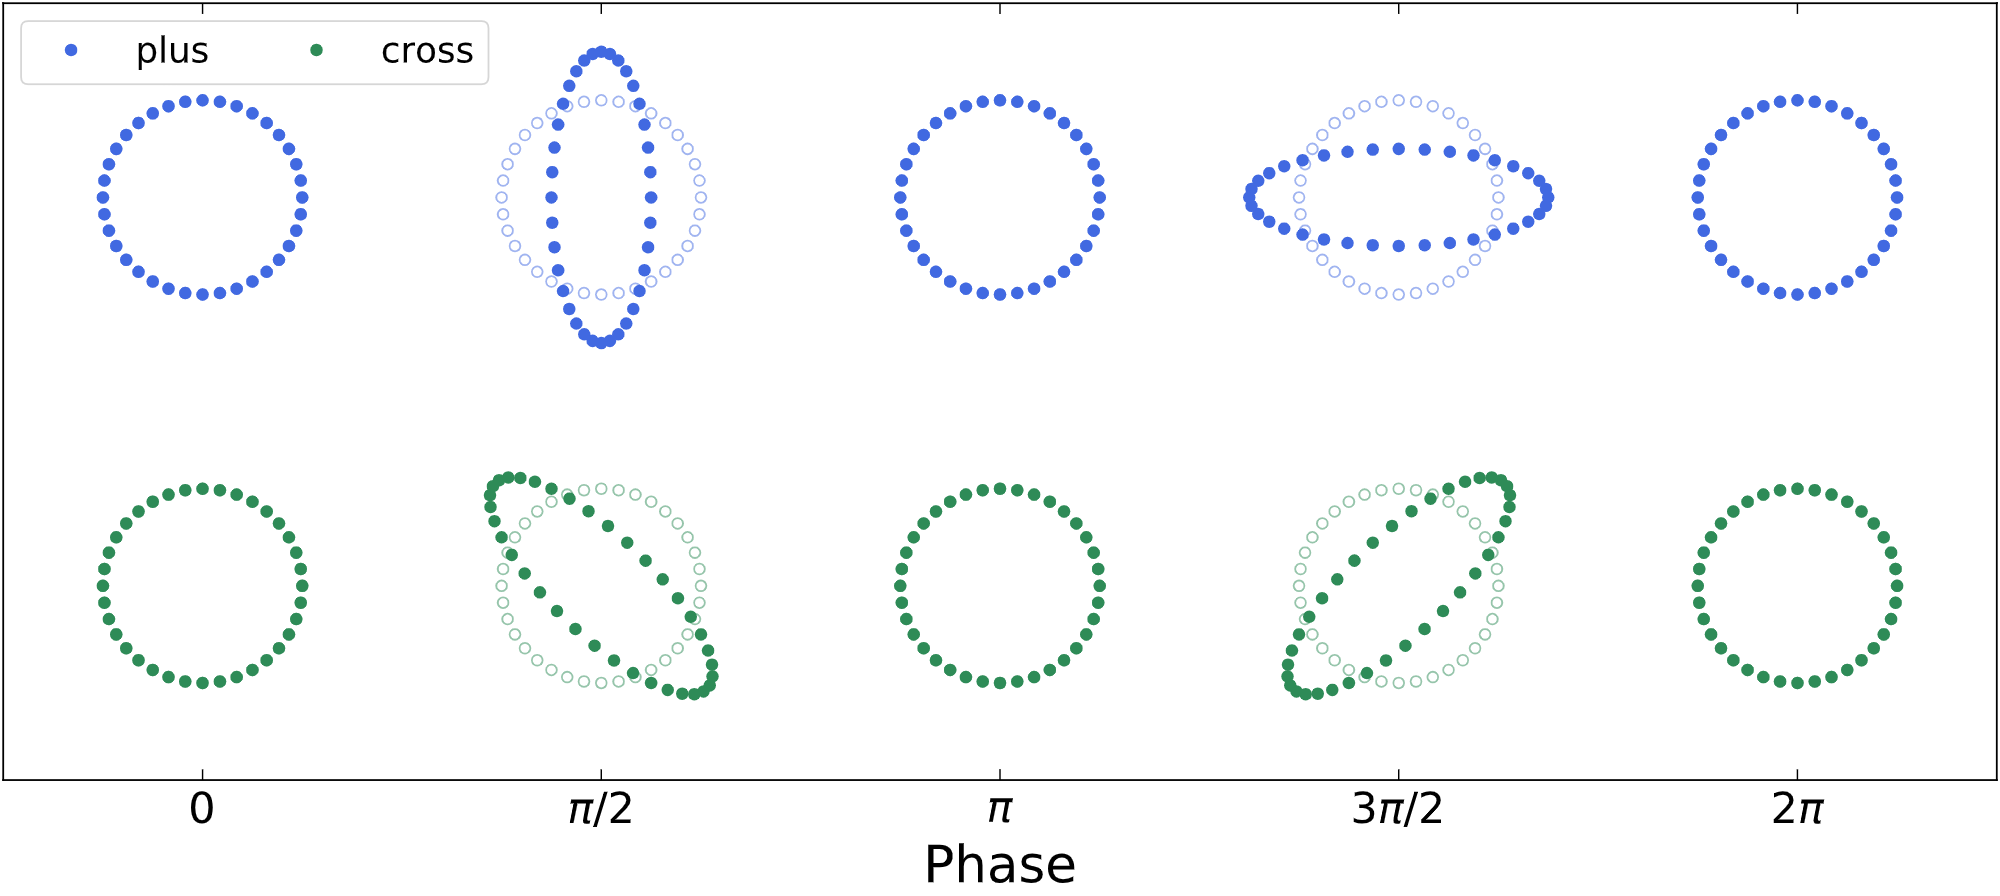
\includegraphics[width=\textwidth]{images/1_general_relativity/polarization.png}
   \caption{\label{fig:polarization}The effect of the two polarizations on a ring of test particles~\cite{gw_polarization_plots}.}
\end{figure}

A \gw polarized completely in the `plus' plane will produce a physical separation of any particle from the centre of the ring of:

\begin{equation}
   \Delta s = R[1 + \frac{1}{2} A_+ \cos(\omega t) \cos(2 \theta)]
   \label{eqn:plus_separation}
\end{equation}

Where $\Delta s$ is the physical separation of the particle from the centre, $R$ is the radius of the circle and, $\theta$ is the polar angle of each particle.

Likewise for a \gw completely polarized in the `cross' plane:

\begin{equation}
   \Delta s = R[1 + \frac{1}{2} A_{\times} \cos(\omega t) \sin(2 \theta)]
   \label{eqn:cross_separation}
\end{equation}

It is important to note that we are treating the separation between the particles and the centre in cartesian coordinates as the TT gauge is a comoving coordinate system where the coordinates of the particles are fixed
even as a \gw passes through.

\section{\label{sec:CBC}Gravitational Wave Sources - Compact Binary Coalescence}

A \cbc occurs when two stellar remnants, such as neutron stars (NSs) or black holes (BHs), in a binary system merge. This section will discuss \cbcs (CBCs) as a source of \gws.

The fraction of stars in binary systems is dependent on mass, research suggests that among very massive stars 80\% might be multiple-star systems \cite{binary_fraction:2006}. This is important as we look for black-hole binary (BBH) systems as one of the CBC sources of \gws. It is also worth mentioning that while most binary systems will form that way, there is the potential for a dynamic capture to occur where compact objects are flung and caught from
their system to other systems; especially in highly dense stellar neighbourhoods such as the centre of galaxies \cite{dynamic_capture:2000}.

Objects emit \gws continuously throughout their lifetimes, causing the orbit of the objects to lose energy and decay. Over the course of billions of years the radius decays until the two objects merge. The \gw frequency is twice that of the orbital frequency \cite{kip_book} and we can determine the frequency sweep (the change in the frequency over time) using the equation (discarding higher order terms for simplicity):

\begin{equation}
   \frac{dF}{dt} = \frac{96}{5 \pi \mathcal{M}^2} (\pi \mathcal{M} F)^{\frac{11}{3}}
   \label{eqn:frequency_sweep}
\end{equation}

Where $F$ is the \gw frequency and $\mathcal{M}$ is the chirp mass: total mass, $M = m_1 + m_2$; reduced mass, $\mu = m_1 m_2/(m_1+m_2)$, symmetric mass ratio $\eta = \mu/M$ then $\mathcal{M} = \eta^\frac{3}{5} M$ \cite{PE:1995}.

Equation \ref{eqn:frequency_sweep} shows that frequency of the \gw changes as a function of both the frequency and the chirp mass of the system. To higher order terms, the frequency evolution depends further on other parameters such as the spin-orbit and spin-spin parameter \cite{CBC_spin:1993}.

For a BBH in a circular orbit, the evolution of the system will depend on 8 parameters: the two masses and six spin components. Further complexities such as neutron stars (non-rigid bodies) or eccentric orbits will require more parameters.

\section{\label{sec:IFOs}Gravitational Wave Detection}

The detection of \gws is made possible by \gw observatories: LIGO consists of Hanford \& Livingston \cite{aLIGO:2015}; Virgo in Pisa \cite{aVirgo:2015}; KAGRA in Japan \cite{KAGRA:2021}; and GEO in Germany \cite{GEO600:2002}. This section will focus on
the design of the LIGO interferometers however, the techniques are similar for all detectors. The configuration of \aligo (aLIGO) is described in detail in the 2016 paper \cite{aLIGO:2015}.

\subsection{\label{sec:laser_interferometry}Laser Interferometry}

As seen in section \ref{sec:Mechanics}, the effects of \gws in cartesian coordinates is a stretching and squeezing of the ring of test particles. We can measure this using laser interferometry allowing the detection of the small
perturbations caused by the presence of \gws in spacetime.

We begin with a basic L-shaped Michelson interferometer, seen in figure \ref{fig:basic_michelson}:

\begin{figure}
   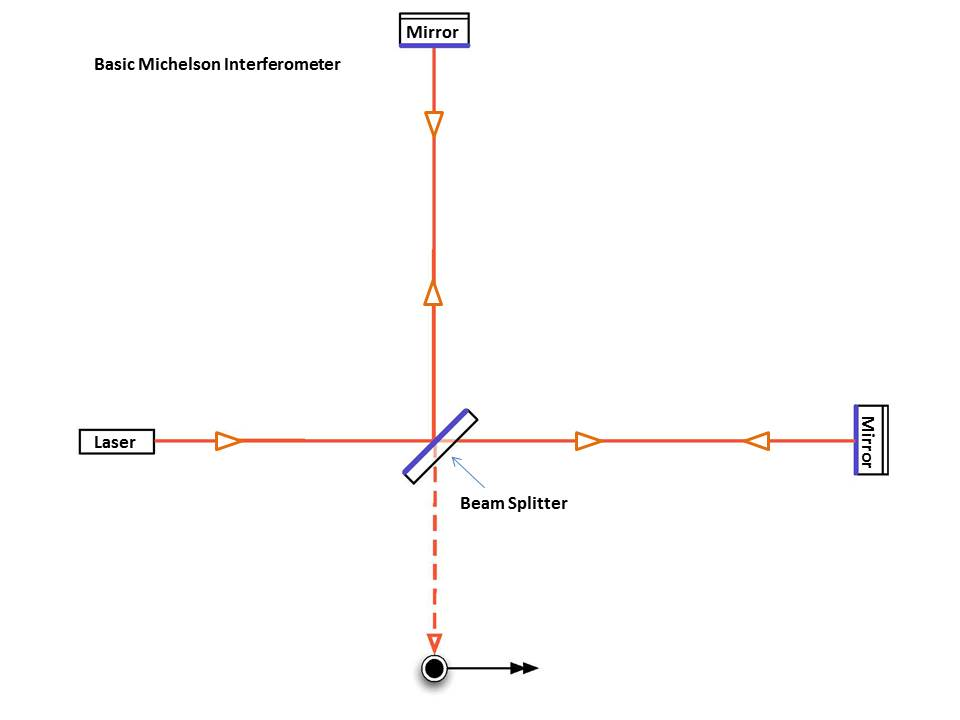
\includegraphics[width=\textwidth]{images/1_general_relativity/Basic_michelson_labeled.jpg}
   \caption{\label{fig:basic_michelson}A basic Michelson interferometer \cite{ligo_ifo}: A laser beam is shone at a beam splitter, the components are sent down equal length perpendicular arms where they reflect off the mirrors at the end, the components are then recombined back at the beam splitter and passed through to the photodetector (black circle) where the interference pattern of the laser is observed.}
\end{figure}

The LIGO detectors are identical in design with arm lengths of 4km, longer arms are able to make more precise measurements, looking at equations \ref{eqn:plus_separation} \& \ref{eqn:cross_separation}, the separation
$\Delta s$ depends on the radius $R$ (analogous to our arm length). We can further increase the distance our laser beam travels by using Fabry-Perot cavities to constantly recycle the laser in the arms. Figure \ref{fig:FP_michelson} shows the inclusion of Fabry-Perot cavities onto our basic Michelson interferometer.

\begin{figure}
   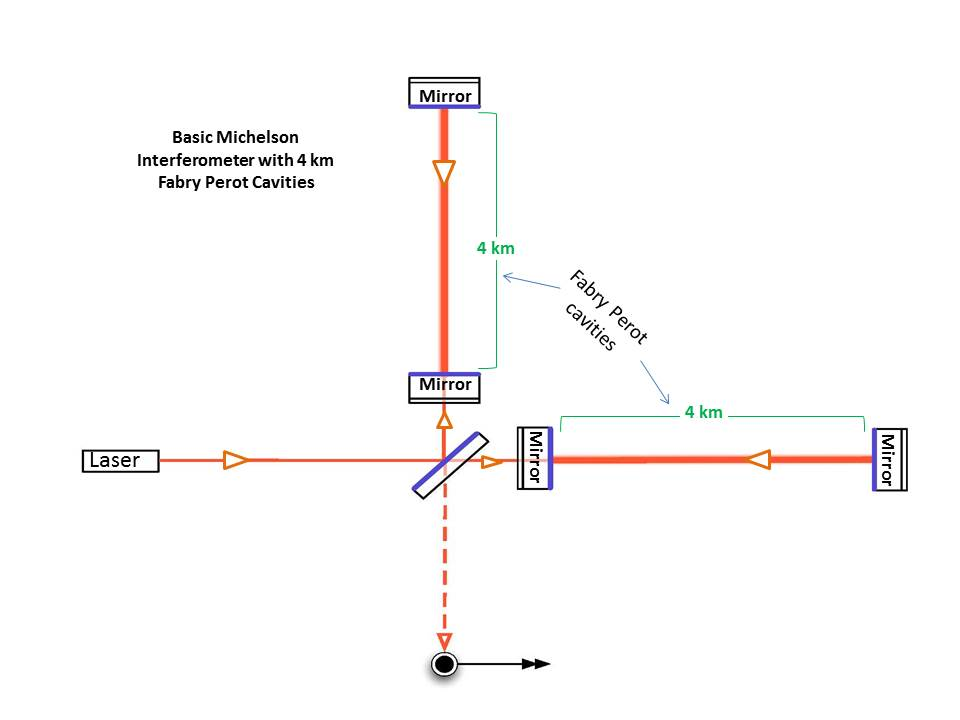
\includegraphics[width=\textwidth]{images/1_general_relativity/Basic_michelson_with_FP_labeled.jpg}
   \caption{\label{fig:FP_michelson}Fabry-Perot cavities \cite{ligo_ifo}: Additional mirrors are placed close to the beam splitter in each arm to allow the laser to traverse the arms many more times, effectively adding distance to our arms.}
\end{figure}

To create Fabry-Perot cavities extra mirrors are placed in each arm close to the beam splitter, these mirrors allow the laser to bounce back and forth within the arm many more times - effectively increasing the distance the laser has travelled. The Fabry-Perot cavities are fully evacuated, further reducing noise from the effects of interactions with particles in the air.

Laser power is continuously built up during this process, the more photons we have in our detector, the greater the resolution at our photodetector. We need to reach a laser power much higher than at the source, the Fabry-Perot
cavities don't provide enough amplification so we need to implement power recycling mirrors prior to the laser reaching the beam splitter. Some of the light from the laser is reflected towards the photodetector from the beam
splitter, the rest of it is sent back to the power recycling mirror. The power recycling mirrors can be seen in figure \ref{fig:IFO}.

\begin{figure}
   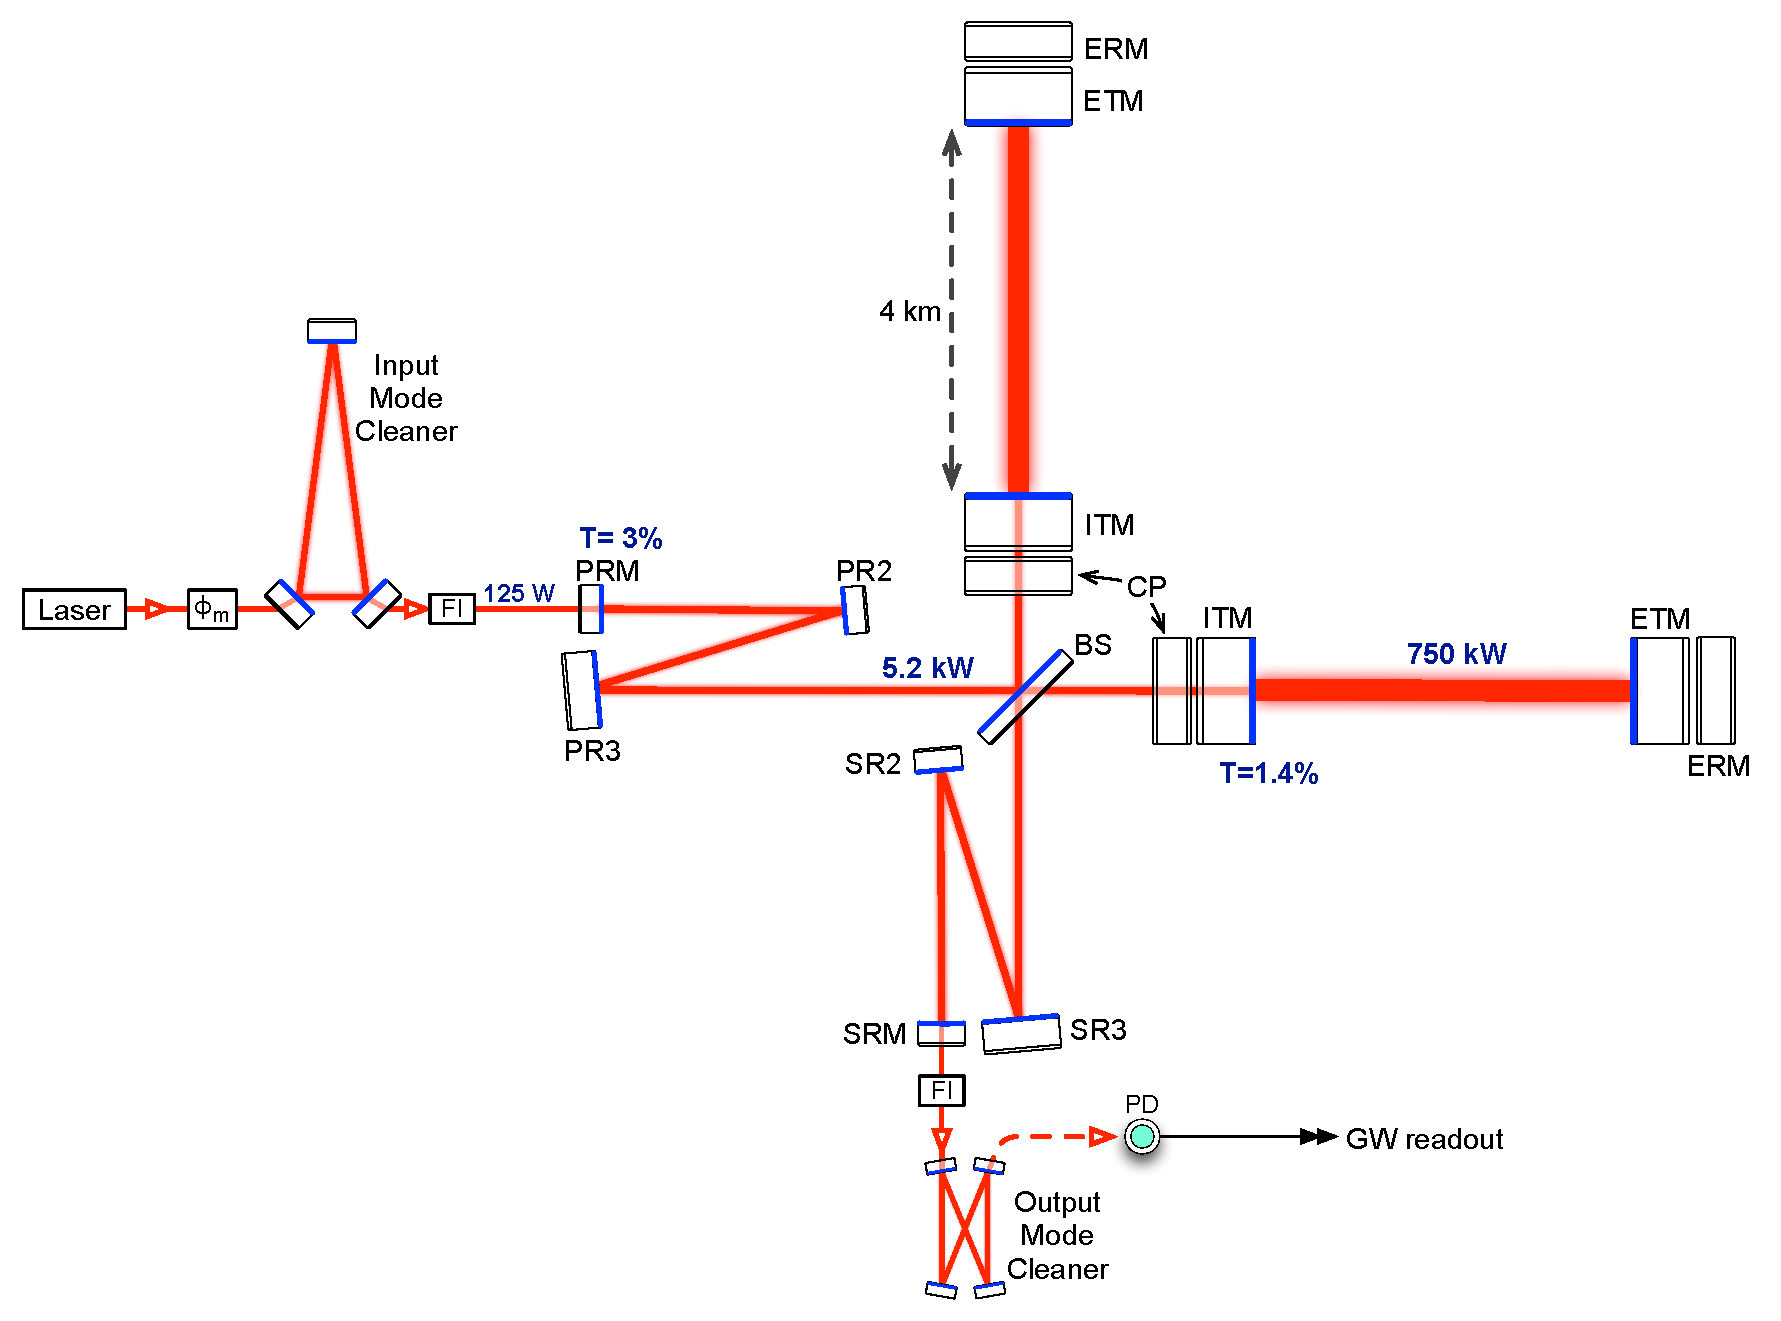
\includegraphics[width=\textwidth]{images/1_general_relativity/IFOdiagram.pdf}
   \caption{\label{fig:IFO}A more complex interferometer diagram \cite{aLIGO:2015}: The Fabry-Perot cavities are formed by the input test mass (ITM) and end test mass (ERM) of each arm, the power recycling mirrors (PRM, PR2, PR3) appear prior to the beam splitter (BS)}
\end{figure}

Within the reference frame of the beam splitter and in the absence of \gws, the distance each laser travels up the arms is equal so that upon returning to the beam splitter, we see a constant interference pattern in the photodetector.
As a \gw propagates through the detector the beam splitter remains at rest but the mirrors at the end of each arm move (in our cartesian coordinate system), the lengths of the arms are now different and the recombination of the two beams will produce a phase difference upon returning back to the beam splitter \cite{thorne_lecture}.
